\documentclass{article}
\usepackage{amssymb,amsmath}
\usepackage{ifxetex,ifluatex}
\ifxetex
  \usepackage{fontspec,xltxtra,xunicode}
  \defaultfontfeatures{Mapping=tex-text,Scale=MatchLowercase}
\else
  \ifluatex
    \usepackage{fontspec}
    \defaultfontfeatures{Mapping=tex-text,Scale=MatchLowercase}
  \else
    \usepackage[utf8]{inputenc}
  \fi
\fi
\usepackage{ctable}
\usepackage{float} % provides the H option for float placement
\usepackage{graphicx}
% We will generate all images so they have a width \maxwidth. This means
% that they will get their normal width if they fit onto the page, but
% are scaled down if they would overflow the margins.
\makeatletter
\def\maxwidth{\ifdim\Gin@nat@width>\linewidth\linewidth
\else\Gin@nat@width\fi}
\makeatother
\let\Oldincludegraphics\includegraphics
\renewcommand{\includegraphics}[1]{\Oldincludegraphics[width=\maxwidth]{#1}}
\ifxetex
  \usepackage[setpagesize=false, % page size defined by xetex
              unicode=false, % unicode breaks when used with xetex
              xetex]{hyperref}
\else
  \usepackage[unicode=true]{hyperref}
\fi
\hypersetup{breaklinks=true, pdfborder={0 0 0}}
\setlength{\parindent}{0pt}
\setlength{\parskip}{6pt plus 2pt minus 1pt}
\setlength{\emergencystretch}{3em}  % prevent overfull lines
\setcounter{secnumdepth}{0}

\title{Descriptives}
\author{Rapport package team @ https://github.com/aL3xa/rapport}
\date{2011--04--26 20:25 CET}

\begin{document}
\maketitle

\subsection{Description}

This template will return descriptive statistics of numerical, or
frequency tables of categorical variables.

\subsubsection{\emph{gender} (``Gender'')}

The dataset has 709 observations with 709 valid values (missing: 0) in
\emph{gender} (``Gender''). This variable seems to be a factor.

\paragraph{Base statistics}

\ctable[pos = H, center, botcap]{llllll}
{% notes
}
{% rows
\FL
 & \textbf{gender} & \textbf{N} & \textbf{pct} & \textbf{cumul.count} & \textbf{cumul.pct}
\ML
1 & male & 432.00 & 60.93 & 432.00 & 60.93
\\\noalign{\medskip}
2 & female & 277.00 & 39.07 & 709.00 & 100.00
\\\noalign{\medskip}
Total &  & 709.00 & 100.00 & 709.00 & 100.00
\LL
}

\paragraph{Barplot}

\begin{figure}[htbp]
\centering
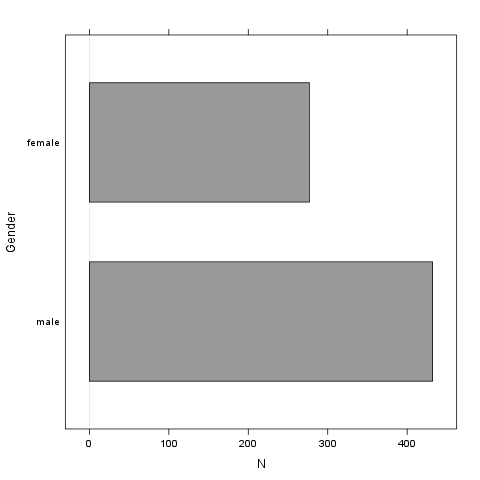
\includegraphics{2a42fb1eb44bf1361b44216c6b0c16ee.png}
\caption{}
\end{figure}

It seems that the highest value is 2 which is exactly 2 times higher
than the smallest value (1).

\subsubsection{\emph{age} (``Age'')}

The dataset has 709 observations with 709 valid values (missing: 0) in
\emph{age} (``Age''). This variable seems to be numeric.

\paragraph{Base statistics}

\ctable[pos = H, center, botcap]{llll}
{% notes
}
{% rows
\FL
\textbf{value} & \textbf{mean(age)} & \textbf{sd(age)} & \textbf{var(age)}
\ML
(all) & 24.56 & 6.84 & 46.78
\LL
}

\paragraph{Histogram}

\begin{figure}[htbp]
\centering
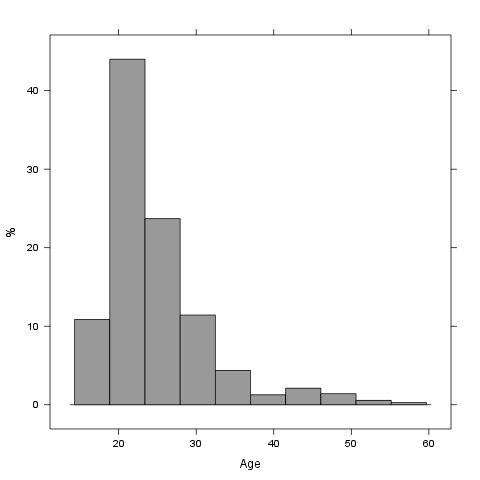
\includegraphics{76fc57f9d2387aff730be60323f25624.png}
\caption{}
\end{figure}

It seems that the highest value is 58 which is exactly 3.625 times
higher than the smallest value (16).

The standard deviation is 6.8399 (variance: 46.784). The expected value
is around 24.557, somewhere between 24.054 and 25.061 (SE: 0.2569).

If we suppose that \emph{Age} is not near to a normal distribution
(test: , skewness: 1.9568, kurtosis: 7.6428), checking the median (23)
might be a better option instead of the mean. The interquartile range
(6) measures the statistics dispersion of the variable (similar to
standard deviation) based on median.

\subsection{Description}

This template will return descriptive statistics of numerical, or
frequency tables of categorical variables.

\subsubsection{\emph{chatim} (``Chat \& IM usage'')}

The dataset has 709 observations with 709 valid values (missing: 0) in
\emph{chatim} (``Chat \& IM usage''). This variable seems to be a
factor.

\paragraph{Base statistics}

\ctable[pos = H, center, botcap]{llllll}
{% notes
}
{% rows
\FL
 & \textbf{chatim} & \textbf{N} & \textbf{pct} & \textbf{cumul.count} & \textbf{cumul.pct}
\ML
1 & never & 64.00 & 9.03 & 64.00 & 9.03
\\\noalign{\medskip}
2 & very rarely & 78.00 & 11.00 & 142.00 & 20.03
\\\noalign{\medskip}
3 & rarely & 65.00 & 9.17 & 207.00 & 29.20
\\\noalign{\medskip}
4 & sometimes & 124.00 & 17.49 & 331.00 & 46.69
\\\noalign{\medskip}
5 & often & 142.00 & 20.03 & 473.00 & 66.71
\\\noalign{\medskip}
6 & very often & 94.00 & 13.26 & 567.00 & 79.97
\\\noalign{\medskip}
7 & always & 142.00 & 20.03 & 709.00 & 100.00
\\\noalign{\medskip}
Total &  & 709.00 & 100.00 & 709.00 & 100.00
\LL
}

\paragraph{Barplot}

\begin{figure}[htbp]
\centering
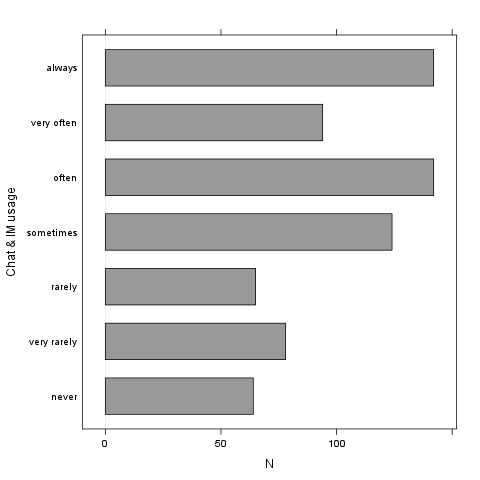
\includegraphics{18ee2d4410677e2bbc343a9a4889cc97.png}
\caption{}
\end{figure}

It seems that the highest value is 7 which is exactly 7 times higher
than the smallest value (1).

\subsubsection{\emph{game} (``On-line games usage'')}

The dataset has 709 observations with 709 valid values (missing: 0) in
\emph{game} (``On-line games usage''). This variable seems to be a
factor.

\paragraph{Base statistics}

\ctable[pos = H, center, botcap]{llllll}
{% notes
}
{% rows
\FL
 & \textbf{game} & \textbf{N} & \textbf{pct} & \textbf{cumul.count} & \textbf{cumul.pct}
\ML
1 & never & 368.00 & 51.90 & 368.00 & 51.90
\\\noalign{\medskip}
2 & very rarely & 132.00 & 18.62 & 500.00 & 70.52
\\\noalign{\medskip}
3 & rarely & 35.00 & 4.94 & 535.00 & 75.46
\\\noalign{\medskip}
4 & sometimes & 65.00 & 9.17 & 600.00 & 84.63
\\\noalign{\medskip}
5 & often & 38.00 & 5.36 & 638.00 & 89.99
\\\noalign{\medskip}
6 & very often & 37.00 & 5.22 & 675.00 & 95.20
\\\noalign{\medskip}
7 & always & 34.00 & 4.80 & 709.00 & 100.00
\\\noalign{\medskip}
Total &  & 709.00 & 100.00 & 709.00 & 100.00
\LL
}

\paragraph{Barplot}

\begin{figure}[htbp]
\centering
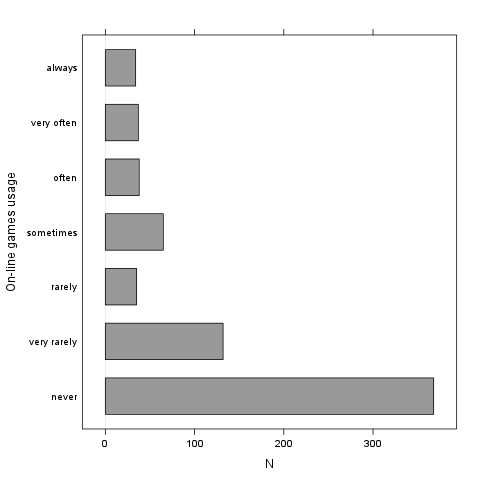
\includegraphics{db92f166fe1966dbd5c6f0b909c181b2.png}
\caption{}
\end{figure}

It seems that the highest value is 7 which is exactly 7 times higher
than the smallest value (1).

\subsubsection{\emph{surf} (``Web surfing usage'')}

The dataset has 709 observations with 709 valid values (missing: 0) in
\emph{surf} (``Web surfing usage''). This variable seems to be a factor.

\paragraph{Base statistics}

\ctable[pos = H, center, botcap]{llllll}
{% notes
}
{% rows
\FL
 & \textbf{surf} & \textbf{N} & \textbf{pct} & \textbf{cumul.count} & \textbf{cumul.pct}
\ML
1 & never & 17.00 & 2.40 & 17.00 & 2.40
\\\noalign{\medskip}
2 & very rarely & 26.00 & 3.67 & 43.00 & 6.06
\\\noalign{\medskip}
3 & rarely & 34.00 & 4.80 & 77.00 & 10.86
\\\noalign{\medskip}
4 & sometimes & 116.00 & 16.36 & 193.00 & 27.22
\\\noalign{\medskip}
5 & often & 164.00 & 23.13 & 357.00 & 50.35
\\\noalign{\medskip}
6 & very often & 151.00 & 21.30 & 508.00 & 71.65
\\\noalign{\medskip}
7 & always & 201.00 & 28.35 & 709.00 & 100.00
\\\noalign{\medskip}
Total &  & 709.00 & 100.00 & 709.00 & 100.00
\LL
}

\paragraph{Barplot}

\begin{figure}[htbp]
\centering
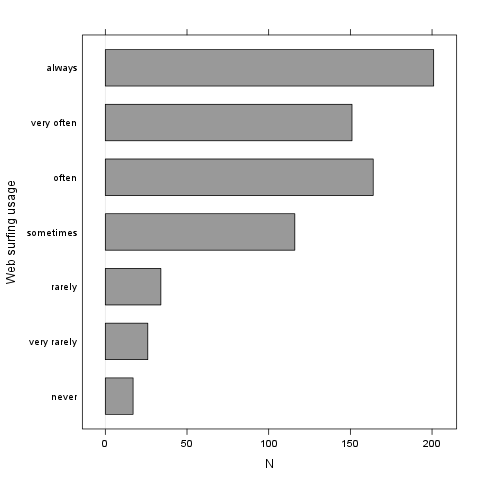
\includegraphics{42a485477f7c7e629c55f3f106b2f482.png}
\caption{}
\end{figure}

It seems that the highest value is 7 which is exactly 7 times higher
than the smallest value (1).

\subsubsection{\emph{email} (``Email usage'')}

The dataset has 709 observations with 709 valid values (missing: 0) in
\emph{email} (``Email usage''). This variable seems to be a factor.

\paragraph{Base statistics}

\ctable[pos = H, center, botcap]{llllll}
{% notes
}
{% rows
\FL
 & \textbf{email} & \textbf{N} & \textbf{pct} & \textbf{cumul.count} & \textbf{cumul.pct}
\ML
1 & never & 13.00 & 1.83 & 13.00 & 1.83
\\\noalign{\medskip}
2 & very rarely & 38.00 & 5.36 & 51.00 & 7.19
\\\noalign{\medskip}
3 & rarely & 51.00 & 7.19 & 102.00 & 14.39
\\\noalign{\medskip}
4 & sometimes & 90.00 & 12.69 & 192.00 & 27.08
\\\noalign{\medskip}
5 & often & 129.00 & 18.19 & 321.00 & 45.28
\\\noalign{\medskip}
6 & very often & 116.00 & 16.36 & 437.00 & 61.64
\\\noalign{\medskip}
7 & always & 272.00 & 38.36 & 709.00 & 100.00
\\\noalign{\medskip}
Total &  & 709.00 & 100.00 & 709.00 & 100.00
\LL
}

\paragraph{Barplot}

\begin{figure}[htbp]
\centering
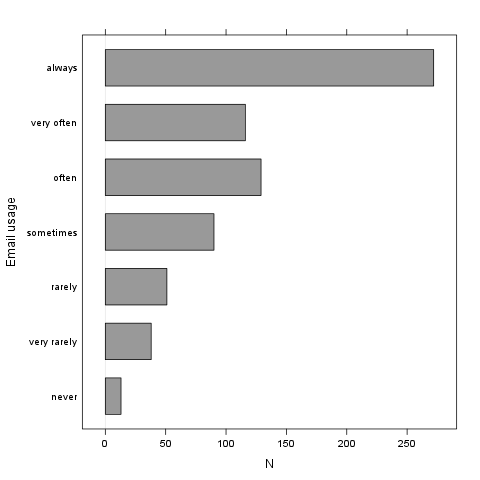
\includegraphics{4271956be974e19ffa2034d316fd201c.png}
\caption{}
\end{figure}

It seems that the highest value is 7 which is exactly 7 times higher
than the smallest value (1).

\subsubsection{\emph{download} (``Download usage'')}

The dataset has 709 observations with 709 valid values (missing: 0) in
\emph{download} (``Download usage''). This variable seems to be a
factor.

\paragraph{Base statistics}

\ctable[pos = H, center, botcap]{llllll}
{% notes
}
{% rows
\FL
 & \textbf{download} & \textbf{N} & \textbf{pct} & \textbf{cumul.count} & \textbf{cumul.pct}
\ML
1 & never & 11.00 & 1.55 & 11.00 & 1.55
\\\noalign{\medskip}
2 & very rarely & 29.00 & 4.09 & 40.00 & 5.64
\\\noalign{\medskip}
3 & rarely & 30.00 & 4.23 & 70.00 & 9.87
\\\noalign{\medskip}
4 & sometimes & 85.00 & 11.99 & 155.00 & 21.86
\\\noalign{\medskip}
5 & often & 130.00 & 18.34 & 285.00 & 40.20
\\\noalign{\medskip}
6 & very often & 171.00 & 24.12 & 456.00 & 64.32
\\\noalign{\medskip}
7 & always & 253.00 & 35.68 & 709.00 & 100.00
\\\noalign{\medskip}
Total &  & 709.00 & 100.00 & 709.00 & 100.00
\LL
}

\paragraph{Barplot}

\begin{figure}[htbp]
\centering
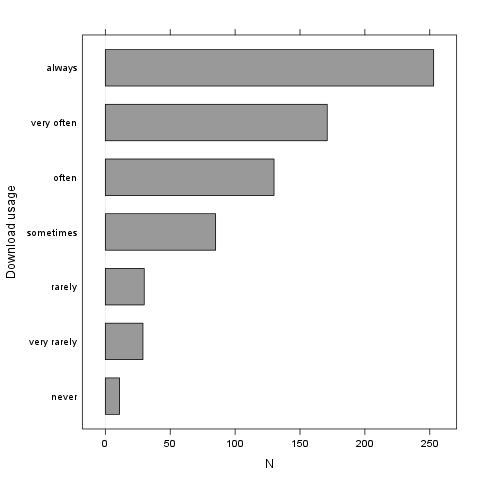
\includegraphics{ec8a2289e719ec679a4abc2f1b3a62ec.png}
\caption{}
\end{figure}

It seems that the highest value is 7 which is exactly 7 times higher
than the smallest value (1).

\subsubsection{\emph{forum} (``Web forums usage'')}

The dataset has 709 observations with 709 valid values (missing: 0) in
\emph{forum} (``Web forums usage''). This variable seems to be a factor.

\paragraph{Base statistics}

\ctable[pos = H, center, botcap]{llllll}
{% notes
}
{% rows
\FL
 & \textbf{forum} & \textbf{N} & \textbf{pct} & \textbf{cumul.count} & \textbf{cumul.pct}
\ML
1 & never & 80.00 & 11.28 & 80.00 & 11.28
\\\noalign{\medskip}
2 & very rarely & 84.00 & 11.85 & 164.00 & 23.13
\\\noalign{\medskip}
3 & rarely & 74.00 & 10.44 & 238.00 & 33.57
\\\noalign{\medskip}
4 & sometimes & 124.00 & 17.49 & 362.00 & 51.06
\\\noalign{\medskip}
5 & often & 112.00 & 15.80 & 474.00 & 66.85
\\\noalign{\medskip}
6 & very often & 125.00 & 17.63 & 599.00 & 84.49
\\\noalign{\medskip}
7 & always & 110.00 & 15.51 & 709.00 & 100.00
\\\noalign{\medskip}
Total &  & 709.00 & 100.00 & 709.00 & 100.00
\LL
}

\paragraph{Barplot}

\begin{figure}[htbp]
\centering
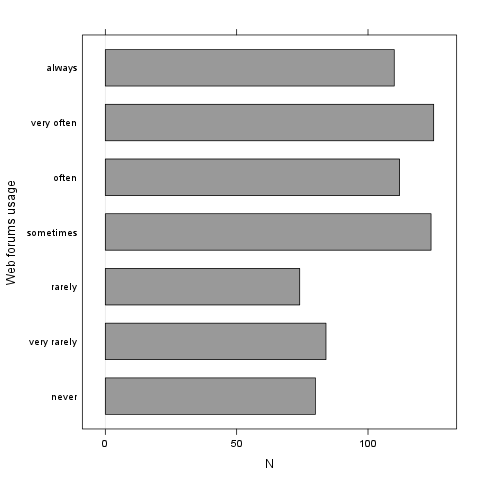
\includegraphics{3f14c76d2ae5a41c21a771f3fd794ca3.png}
\caption{}
\end{figure}

It seems that the highest value is 7 which is exactly 7 times higher
than the smallest value (1).

\subsubsection{\emph{socnet} (``Social networks usage'')}

The dataset has 709 observations with 709 valid values (missing: 0) in
\emph{socnet} (``Social networks usage''). This variable seems to be a
factor.

\paragraph{Base statistics}

\ctable[pos = H, center, botcap]{llllll}
{% notes
}
{% rows
\FL
 & \textbf{socnet} & \textbf{N} & \textbf{pct} & \textbf{cumul.count} & \textbf{cumul.pct}
\ML
1 & never & 210.00 & 29.62 & 210.00 & 29.62
\\\noalign{\medskip}
2 & very rarely & 111.00 & 15.66 & 321.00 & 45.28
\\\noalign{\medskip}
3 & rarely & 59.00 & 8.32 & 380.00 & 53.60
\\\noalign{\medskip}
4 & sometimes & 94.00 & 13.26 & 474.00 & 66.85
\\\noalign{\medskip}
5 & often & 82.00 & 11.57 & 556.00 & 78.42
\\\noalign{\medskip}
6 & very often & 85.00 & 11.99 & 641.00 & 90.41
\\\noalign{\medskip}
7 & always & 68.00 & 9.59 & 709.00 & 100.00
\\\noalign{\medskip}
Total &  & 709.00 & 100.00 & 709.00 & 100.00
\LL
}

\paragraph{Barplot}

\begin{figure}[htbp]
\centering
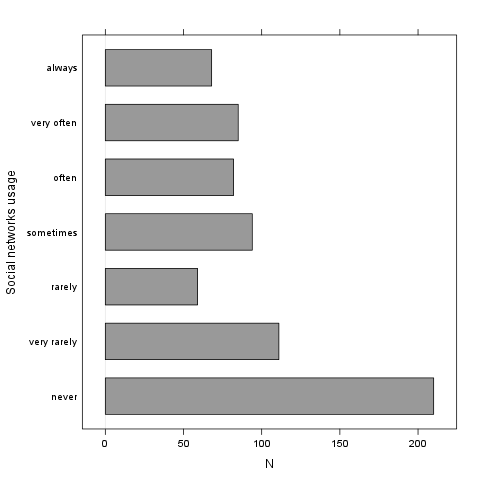
\includegraphics{c1a552be1b3a4299ff06e272129d8096.png}
\caption{}
\end{figure}

It seems that the highest value is 7 which is exactly 7 times higher
than the smallest value (1).

\subsubsection{\emph{xxx} (``Adult sites usage'')}

The dataset has 709 observations with 709 valid values (missing: 0) in
\emph{xxx} (``Adult sites usage''). This variable seems to be a factor.

\paragraph{Base statistics}

\ctable[pos = H, center, botcap]{llllll}
{% notes
}
{% rows
\FL
 & \textbf{xxx} & \textbf{N} & \textbf{pct} & \textbf{cumul.count} & \textbf{cumul.pct}
\ML
1 & never & 293.00 & 41.33 & 293.00 & 41.33
\\\noalign{\medskip}
2 & very rarely & 128.00 & 18.05 & 421.00 & 59.38
\\\noalign{\medskip}
3 & rarely & 55.00 & 7.76 & 476.00 & 67.14
\\\noalign{\medskip}
4 & sometimes & 137.00 & 19.32 & 613.00 & 86.46
\\\noalign{\medskip}
5 & often & 48.00 & 6.77 & 661.00 & 93.23
\\\noalign{\medskip}
6 & very often & 29.00 & 4.09 & 690.00 & 97.32
\\\noalign{\medskip}
7 & always & 19.00 & 2.68 & 709.00 & 100.00
\\\noalign{\medskip}
Total &  & 709.00 & 100.00 & 709.00 & 100.00
\LL
}

\paragraph{Barplot}

\begin{figure}[htbp]
\centering
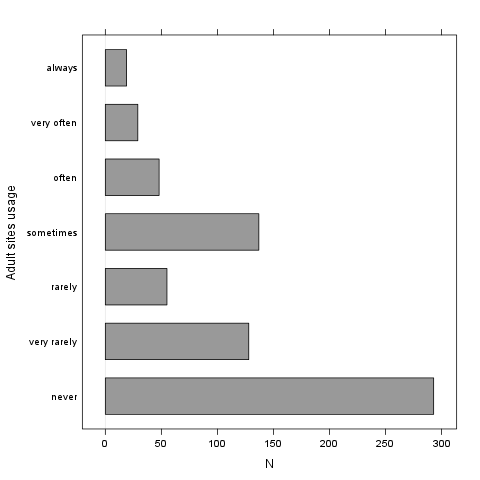
\includegraphics{053614b5b842759f559adcc0da8cc645.png}
\caption{}
\end{figure}

It seems that the highest value is 7 which is exactly 7 times higher
than the smallest value (1).

\end{document}
